Zu Beginn wirkt nur die Gewichtskraft, die Springerin fällt mit $a = g$. Mit zunehmender Geschwindigkeit wächst der Luftwiderstand, die Beschleunigung nimmt ab und geht gegen null, sobald die Endgeschwindigkeit $v_\mathrm{E}$ erreicht ist.

\begin{center}
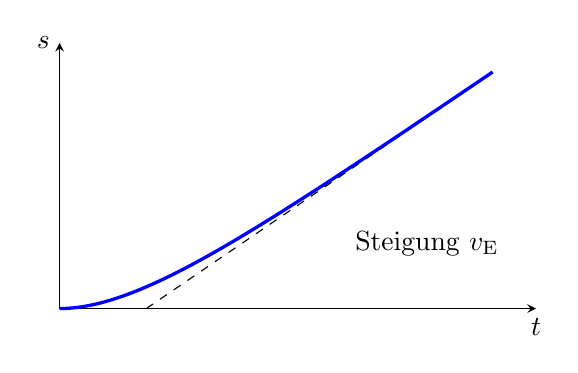
\begin{tikzpicture}[>=stealth, xscale=1.1, yscale=0.75]
 \draw[->] (0,0) -- (5.5,0) node[below] {$t$};
 \draw[->] (0,0) -- (0,4.5) node[left] {$s$};
 \draw[dashed] (1,0) -- (5,4);
 \draw[blue, very thick, domain=0:5, samples=60] plot (\x, {\x-1+exp(-\x)});
 \node[anchor=west] at (3.3,1.1) {Steigung $v_\mathrm{E}$};
\end{tikzpicture}
\hspace{1cm}
\begin{tikzpicture}[>=stealth, xscale=1.1, yscale=0.75]
 \draw[->] (0,0) -- (5.5,0) node[below] {$t$};
 \draw[->] (0,0) -- (0,4.5) node[left] {$a$};
 \draw (0.1,3.5) -- (-0.1,3.5) node[left] {$g$};
 \draw[blue, very thick, domain=0:5, samples=60] plot (\x, {3.5*exp(-\x)});
\end{tikzpicture}
\end{center}

Das $s(t)$-Diagramm beginnt wie beim freien Fall als Parabel mit waagrechter Tangente und geht in eine Gerade mit der Steigung $v_\mathrm{E}$ über (gestrichelt).
